\section{Replacing \code{return} statements}

If the return type of the method is not \code{void}, then an assignment to the \code{ret} variable with the right-hand side
representing the expression of the \code{return} statement is added in the place of the \code{return} statement. Then the
current stack frame is popped from the stack by a call to \code{pop()} on the \code{stack} object. Finally, a
\code{break} statement is added to the parent block of the \code{return} statement. The target of this \code{break}
statement needs to be the \code{switch} statement enclosing the basic blocks. This is why if there is at least one
\code{return} statement in the method which is still included in a statement which can be a \code{break} target
after generating the basic blocks, the \code{switch} statement enclosing the basic blocks is prepended with a label
called \code{switchLabel}. The \code{break} statements corresponding to these \code{return} statements also
have the label \code{switchLabel}. Otherwise, these \code{break} statements would transfer control to the statement after
the enclosing statement and not to the statement after the \code{switch} statement, as it should happen.

An example of this pass is provided in \labelindexref{Figure}{img:return}.

\begin{figure}[htb]
    \makebox[\linewidth][c]{%
    \begin{subfigure}[b]{.6\textwidth}
        \centering
        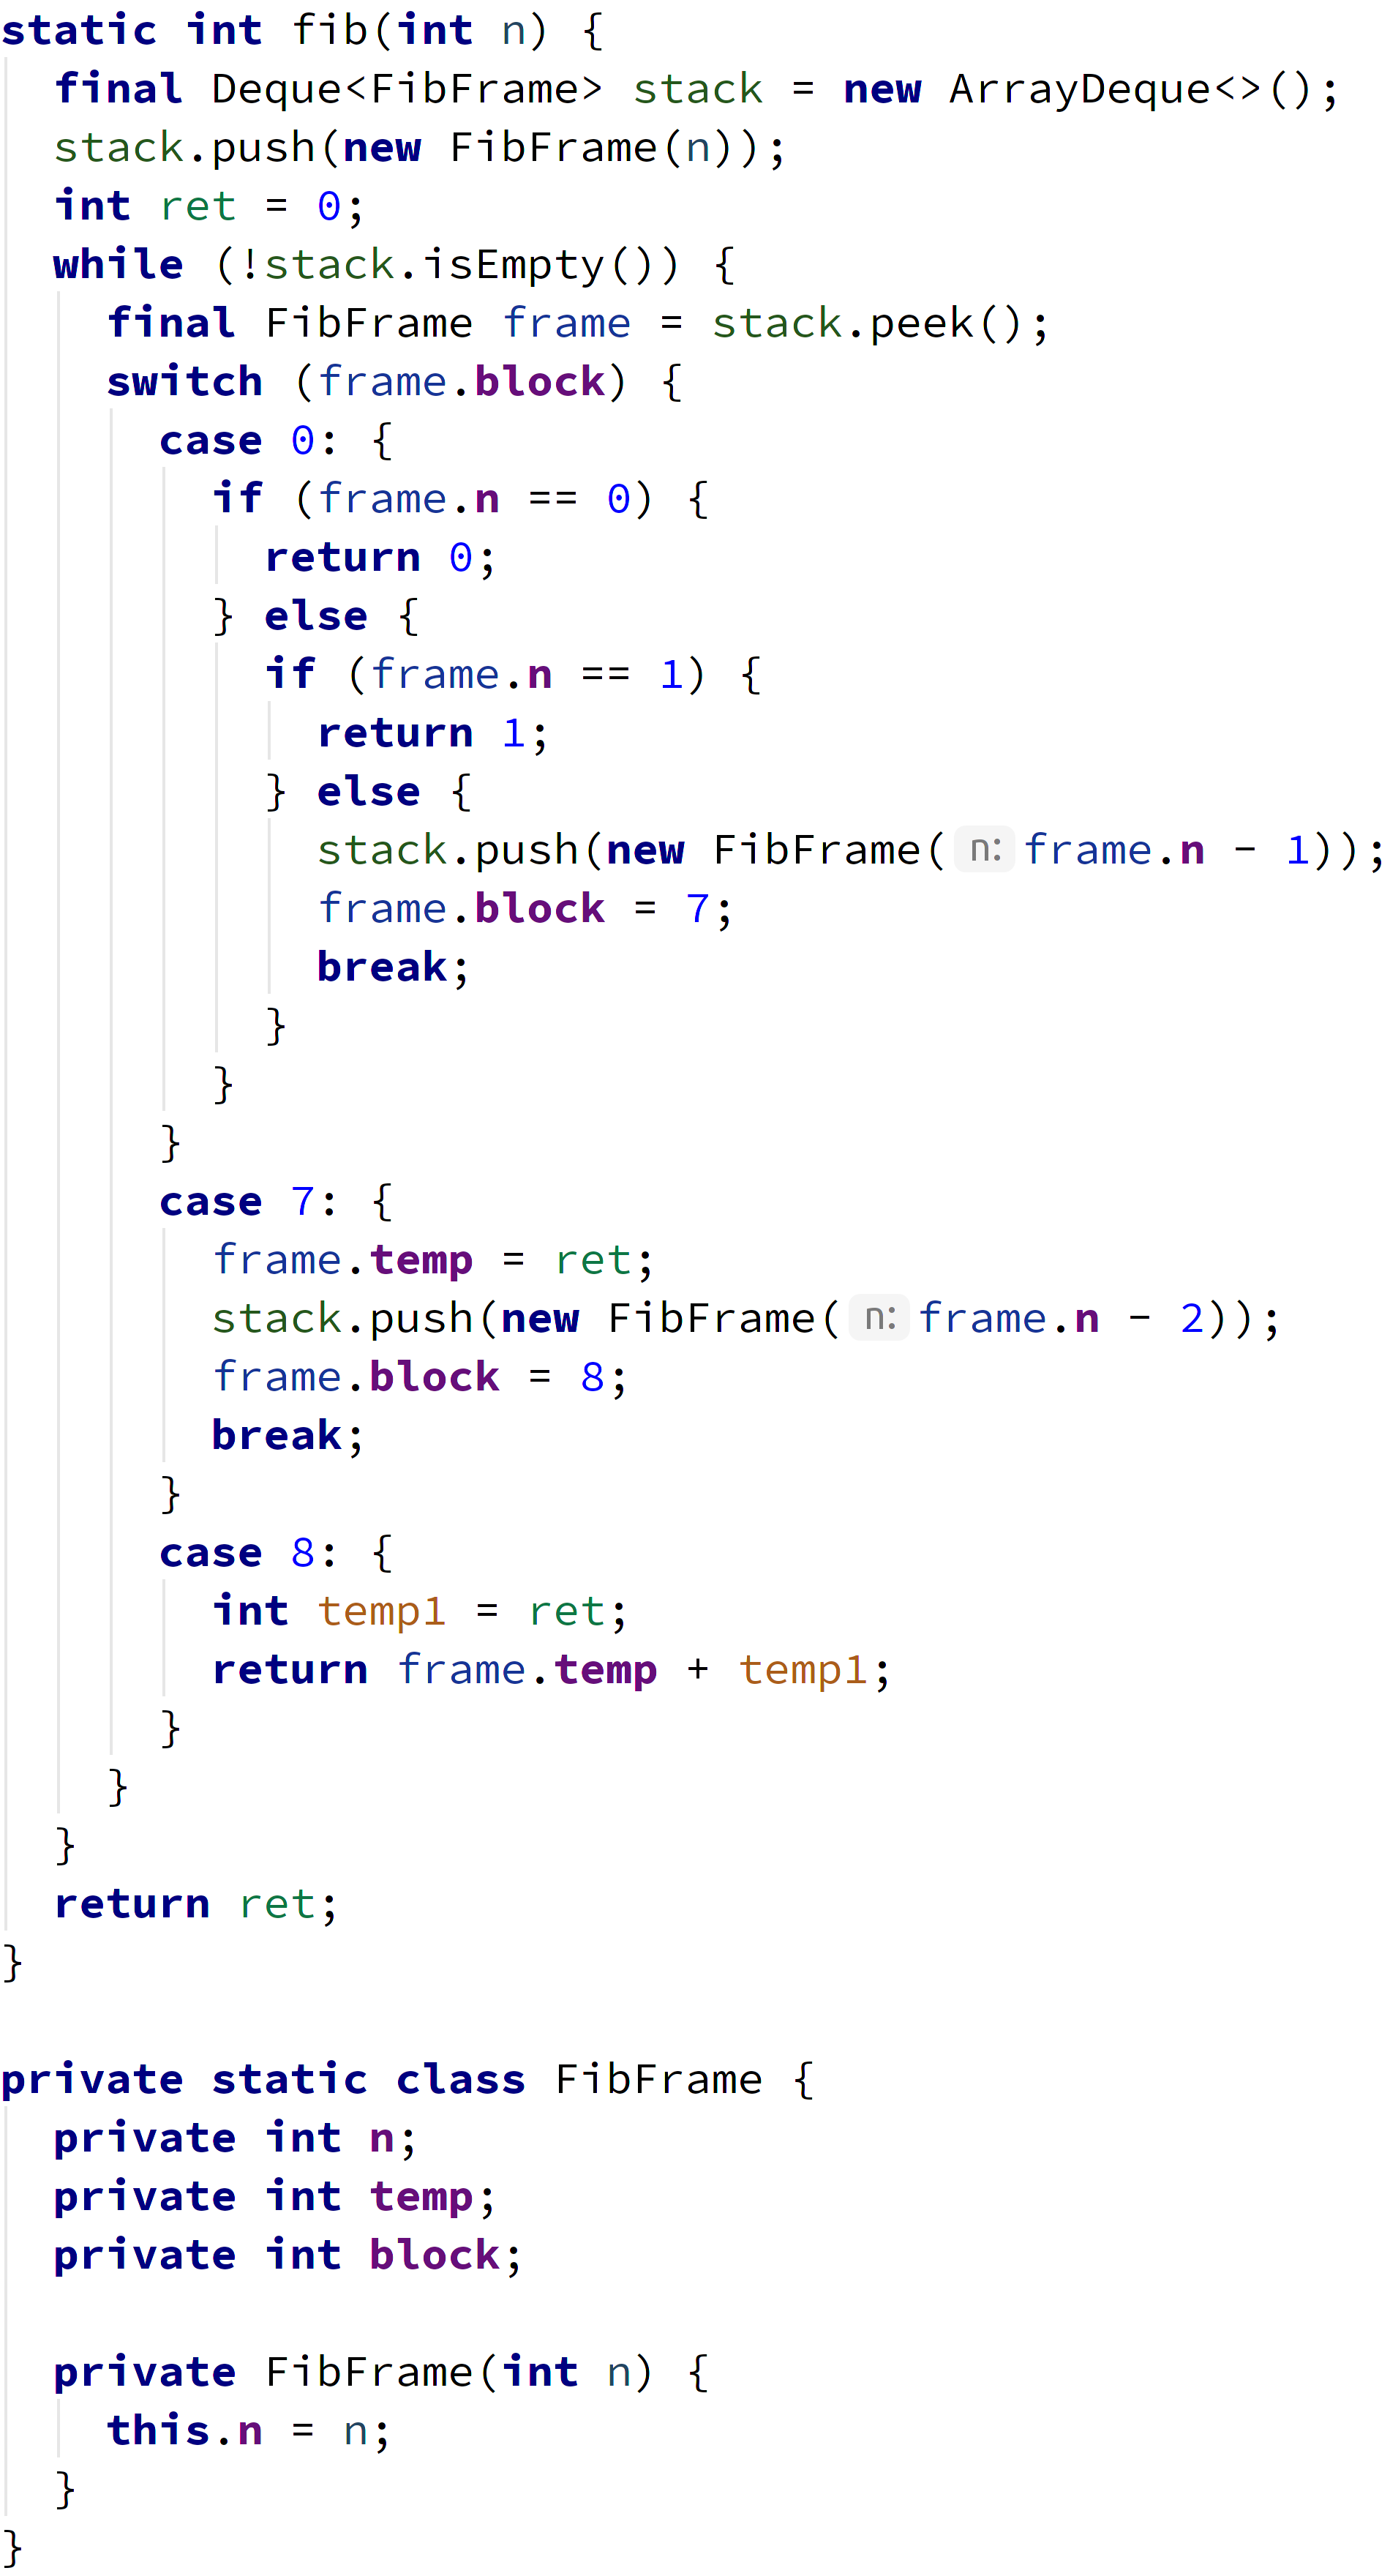
\includegraphics[height=5in]{src/img/inline-blocks-after-white-44.png}
        \caption{Before}
    \end{subfigure}%
    \begin{subfigure}[b]{.6\textwidth}
        \centering
        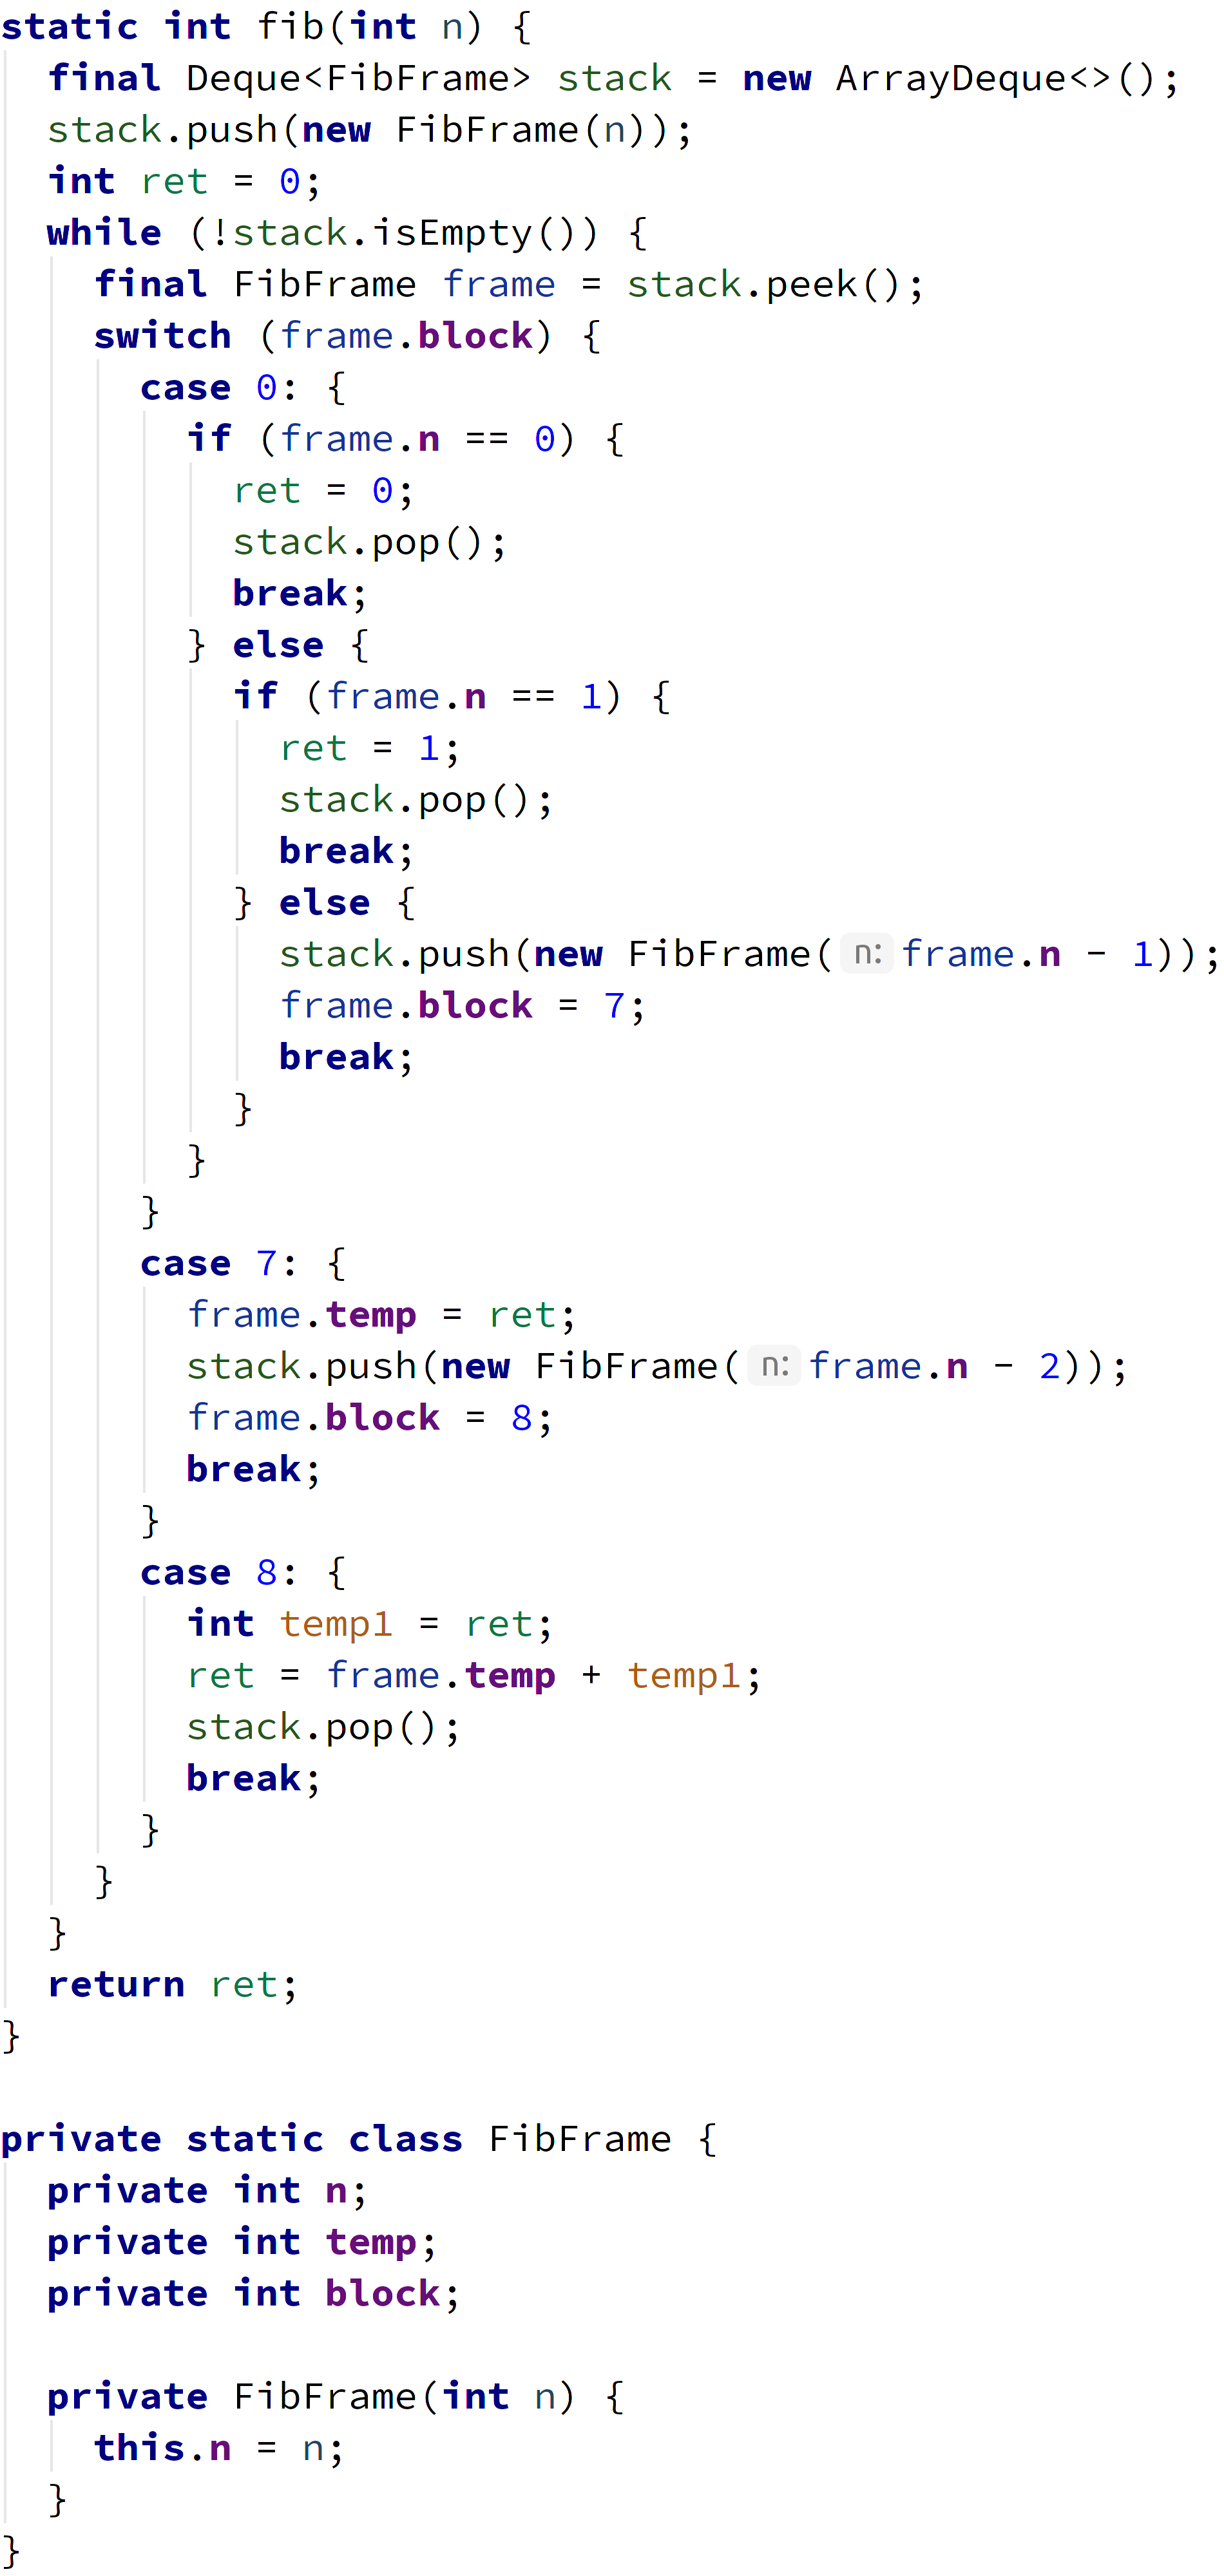
\includegraphics[height=5.682in]{src/img/replace-return-after-50.png}
        \caption{After}
    \end{subfigure}%
    }\\
    \caption{Replacing \code{return} statements \label{img:return}}
\end{figure}